\documentclass[10pt, final]{IEEEtran}
%\documentclass[12pt, final, onecolumn]{IEEEtran}
%\documentclass[journal, final]{IEEEtran}

%allows for using the 1in margins on a page
%\usepackage{fullpage}
%allows for using graphics in the paper
\usepackage{graphicx}
%package needed to set the document into
%double space mode
\usepackage{setspace}
%allows for the use of subfigures
\usepackage{subfigure}
\usepackage{times}
\usepackage[table]{xcolor}
\usepackage{amsthm}
\usepackage{amsmath}
\usepackage{graphicx}
\usepackage{epstopdf}
\usepackage{algpseudocode}
\usepackage{algorithm}
\usepackage{caption}
\usepackage{float}
\usepackage{varwidth}
\usepackage{cite}
%\usepackage{algorithmic}
%\algsetup{linenosize=\small}
%\usepackage{latex8}

%% Define own float style called "algorithm"
%\makeatletter
%\newcommand\fs@algorithm{%
%  \let\@fs@capt\floatc@algorithm
%  \def\@fs@pre{\hrule height.8pt depth0pt\relax}% \kern2pt removed
%  \def\@fs@mid{\hrule\kern2pt}%  \kern2pt removed
%  \def\@fs@post{\kern2pt\hrule\relax}%
%  \let\@fs@iftopcapt\iftrue}
%\makeatother
%
%% Make the algorithm environment use the algorithm float style
%\floatstyle{algorithm}
%\restylefloat{algorithm}
\setlength{\floatsep}{10pt plus 2pt minus 2pt}
\setlength{\textfloatsep}{10pt plus 2pt minus 2pt}
\setlength{\intextsep}{10pt plus 2pt minus 2pt}

% Theorem Styles
\newtheorem{theorem}{Theorem}
\newtheorem{lemma}[theorem]{Lemma}
\newtheorem{proposition}[theorem]{Proposition}
\newtheorem{corollary}[theorem]{Corollary}
% Definition Styles
\theoremstyle{definition}
\newtheorem{definition}{Definition}
\newtheorem{example}{Example}
\theoremstyle{remark}
\newtheorem{remark}{Remark}

\newlength\myindent
\setlength\myindent{2em}
\newcommand\bindent{%
  \begingroup
  \setlength{\itemindent}{\myindent}
  \addtolength{\algorithmicindent}{\myindent}
}
\newcommand\eindent{\endgroup}

\captionsetup[table]{font=small,skip=0pt}
\captionsetup[figure]{font=small,skip=0pt}

%\textwidth 6.0in
%\textheight 8.5in

\textwidth 7in
\textheight 9in

\pagestyle{empty}

%Insert the title of the paper here
%\title{Minimizing Cache Overhead via \\Loaded Cache Blocks and Preemption Placement}
%\title{Optimal Preemption Point Placement \\Using Interdependent Cache Related Preemption Delay}

%authors of the paper
%\author{{John Cavicchio, Corey Tessler, and Nathan Fisher}
%Affiliation
%\vspace{1.6mm}\\
%\fontsize{10}{10}\selectfont\itshape
%Wayne State University\\
%\fontsize{9}{9}\selectfont\ttfamily\upshape
%\{ba6444, corey.tessler, fishern\}@wayne.edu\\}

%in order to remove the date
\date{}


%begin document
\begin{document}


%title
%\maketitle
\pagestyle{plain}

\thispagestyle{empty}
\setcounter{figure}{8}
\setcounter{section}{8}
%
\clearpage
%
\section{Appendix}\label{sec:appendix}
%
\vspace{-20pt}
\begin{figure}[h!]
\begin{center}
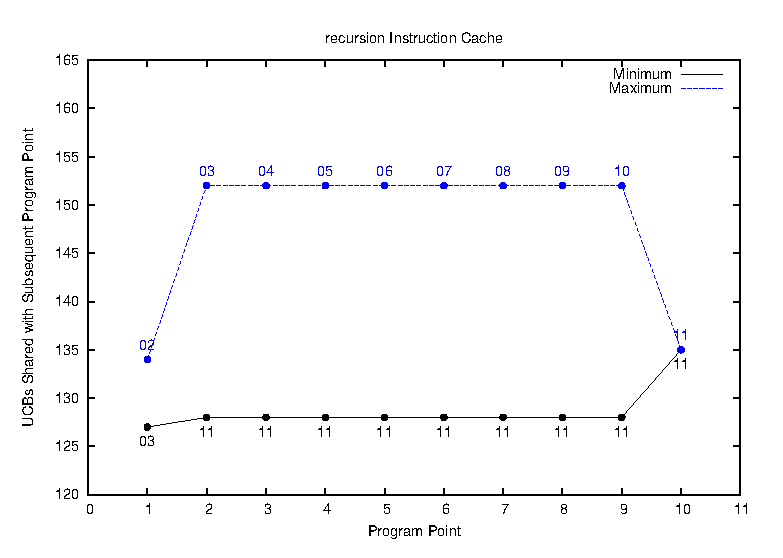
\includegraphics[width=\linewidth]{eps/recursion-icache.eps}
\caption{Recursion Instruction Cache.}
\label{fig:recursion_instruction_cache}
\end{center}
\end{figure}
%
\vspace{-20pt}
\begin{figure}[h!]
\begin{center}
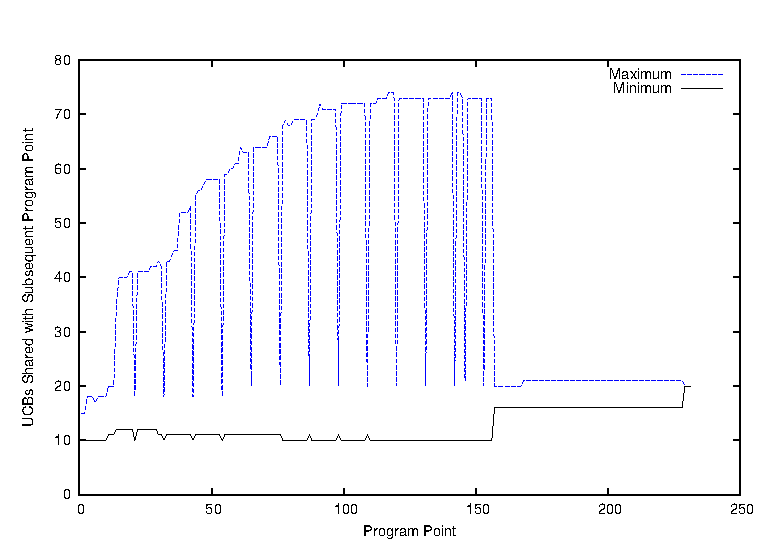
\includegraphics[width=\linewidth]{eps/adpcm-dcache.eps}
\caption{ADPCM Data Cache.}
\label{fig:adpcm_data_cache}
\end{center}
\end{figure}
%
\vspace{-20pt}
\begin{figure}[h!]
\begin{center}
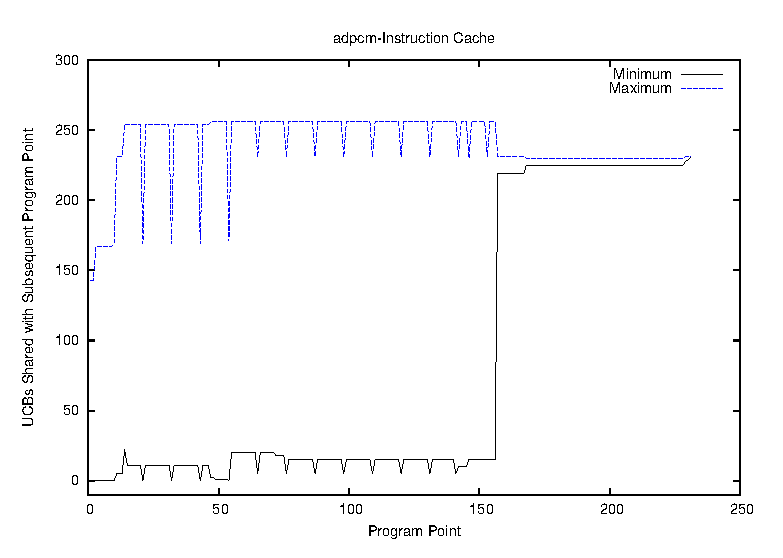
\includegraphics[width=\linewidth]{eps/adpcm-icache.eps}
\caption{ADPCM Instruction Cache.}
\label{fig:adpcm_instruction_cache}
\end{center}
\end{figure}
%
\vspace{-20pt}
\begin{figure}[h!]
\begin{center}
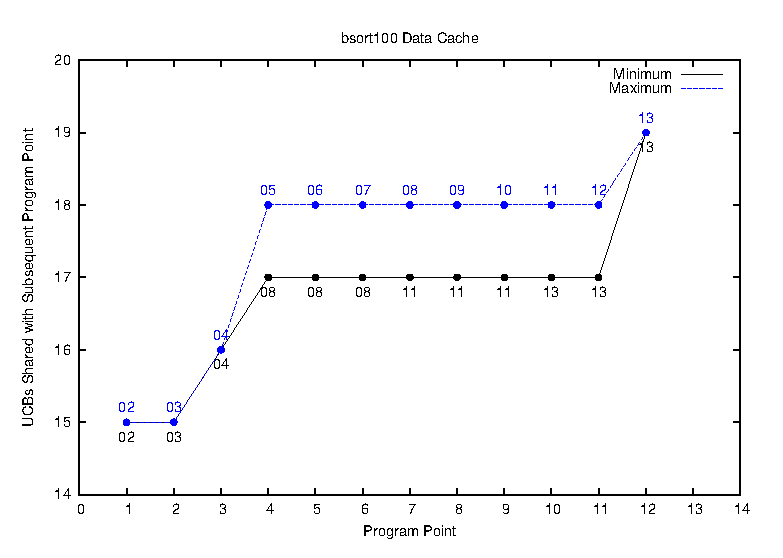
\includegraphics[width=\linewidth]{eps/bsort100-dcache.eps}
\caption{BSORT100 Data Cache.}
\label{fig:bsort100_data_cache}
\end{center}
\end{figure}
%
\vspace{-20pt}
\begin{figure}[h!]
\begin{center}
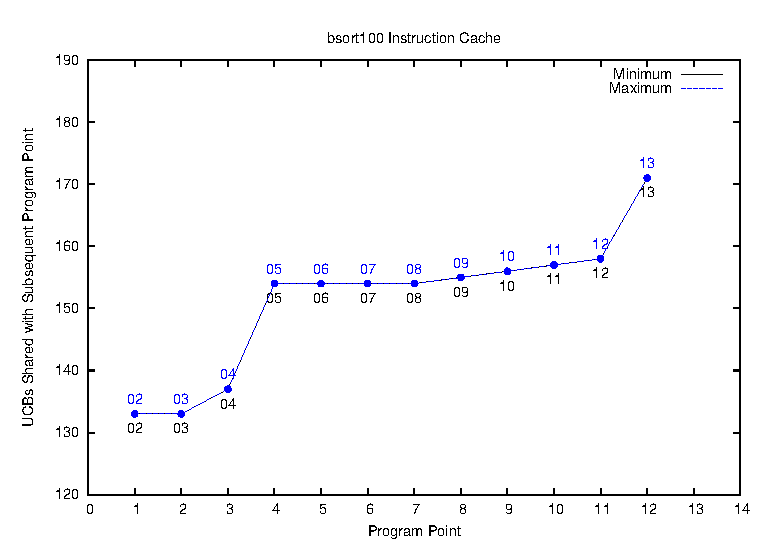
\includegraphics[width=\linewidth]{eps/bsort100-icache.eps}
\caption{BSORT100 Instruction Cache.}
\label{fig:bsort100_instruction_cache}
\end{center}
\end{figure}
%
\vspace{-20pt}
\begin{figure}[h!]
\begin{center}
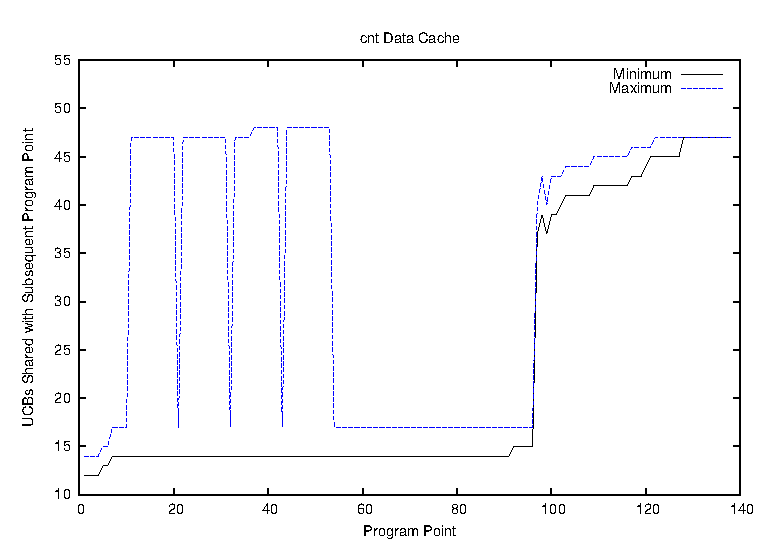
\includegraphics[width=\linewidth]{eps/cnt-dcache.eps}
\caption{CNT Data Cache.}
\label{fig:cnt_data_cache}
\end{center}
\end{figure}
%
\vspace{-20pt}
\begin{figure}[h!]
\begin{center}
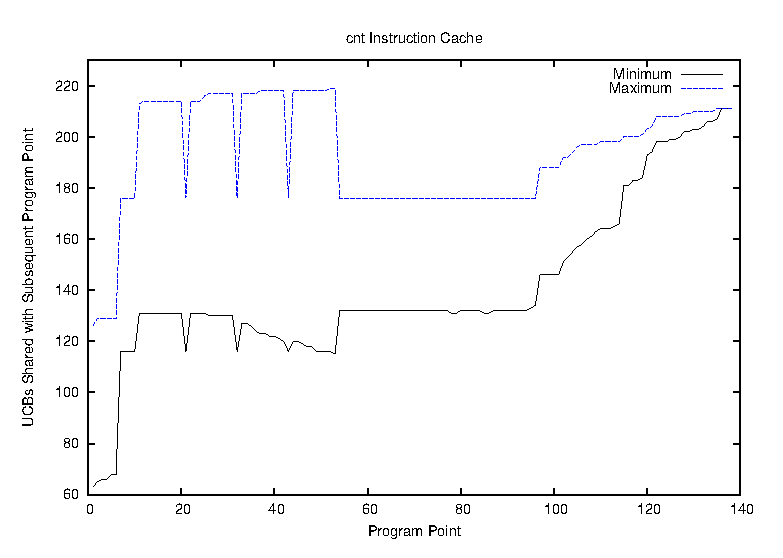
\includegraphics[width=\linewidth]{eps/cnt-icache.eps}
\caption{CNT Instruction Cache.}
\label{fig:cnt_instruction_cache}
\end{center}
\end{figure}
%
\vspace{-20pt}
\begin{figure}[h!]
\begin{center}
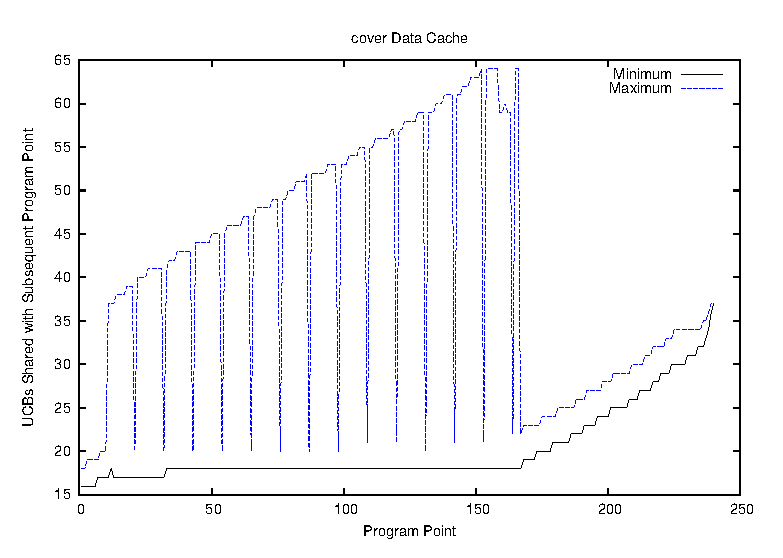
\includegraphics[width=\linewidth]{eps/cover-dcache.eps}
\caption{Cover Data Cache.}
\label{fig:cover_data_cache}
\end{center}
\end{figure}
%
\vspace{-20pt}
\begin{figure}[h!]
\begin{center}
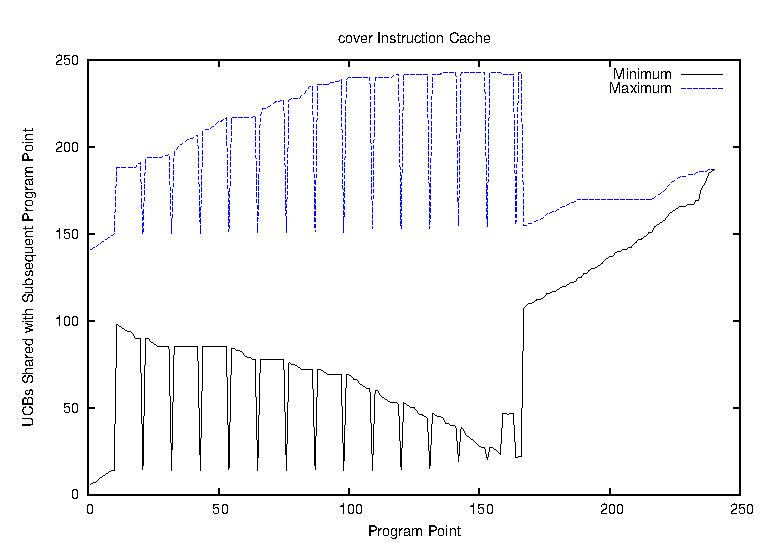
\includegraphics[width=\linewidth]{eps/cover-icache.eps}
\caption{Cover Instruction Cache.}
\label{fig:cover_instruction_cache}
\end{center}
\end{figure}
%
\vspace{-20pt}
\begin{figure}[h!]
\begin{center}
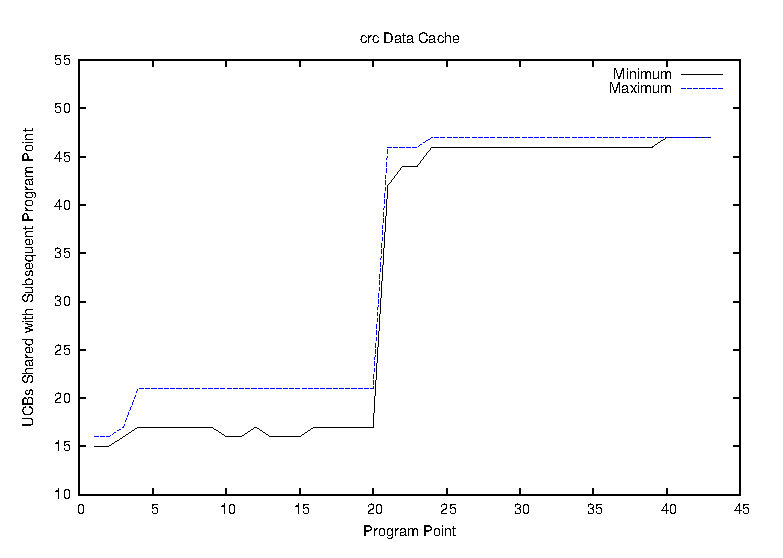
\includegraphics[width=\linewidth]{eps/crc-dcache.eps}
\caption{CRC Data Cache.}
\label{fig:crc_data_cache}
\end{center}
\end{figure}
%
\vspace{-20pt}
\begin{figure}[h!]
\begin{center}
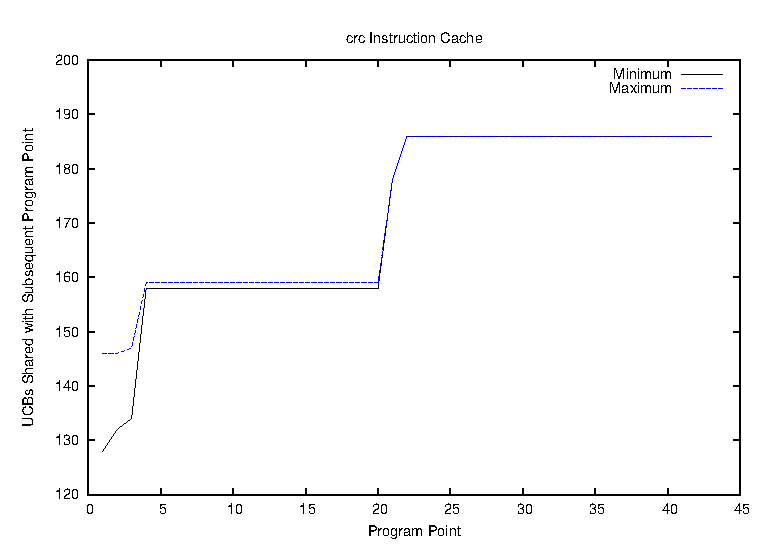
\includegraphics[width=\linewidth]{eps/crc-icache.eps}
\caption{CRC Instruction Cache.}
\label{fig:crc_instruction_cache}
\end{center}
\end{figure}
%
\vspace{-20pt}
\begin{figure}[h!]
\begin{center}
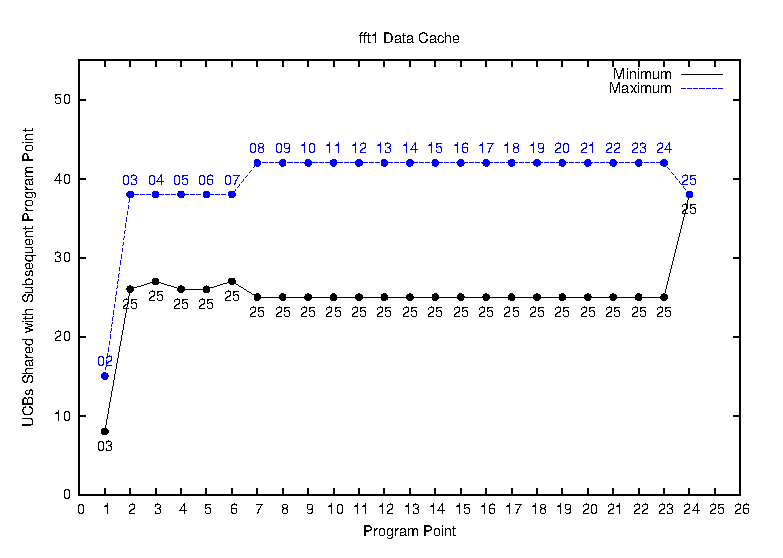
\includegraphics[width=\linewidth]{eps/fft1-dcache.eps}
\caption{FFT1 Data Cache.}
\label{fig:fft1_data_cache}
\end{center}
\end{figure}
%
\vspace{-20pt}
\begin{figure}[h!]
\begin{center}
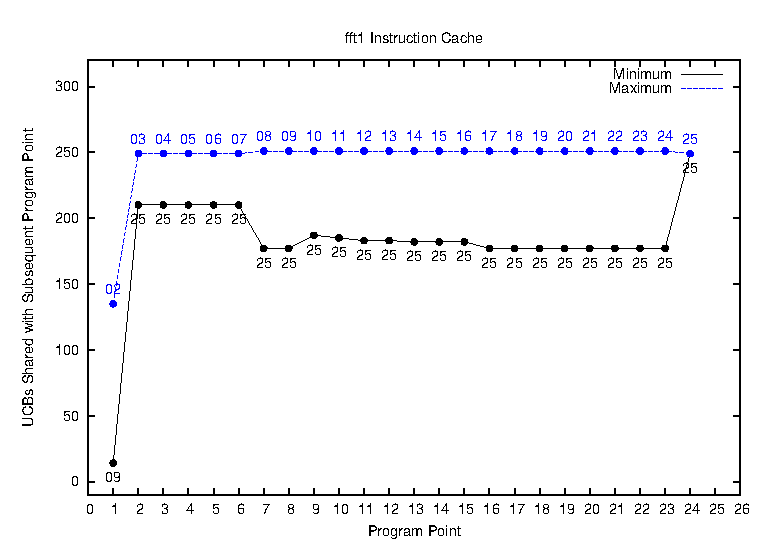
\includegraphics[width=\linewidth]{eps/fft1-icache.eps}
\caption{FFT1 Instruction Cache.}
\label{fig:fft1_instruction_cache}
\end{center}
\end{figure}
%
\vspace{-20pt}
\begin{figure}[h!]
\begin{center}
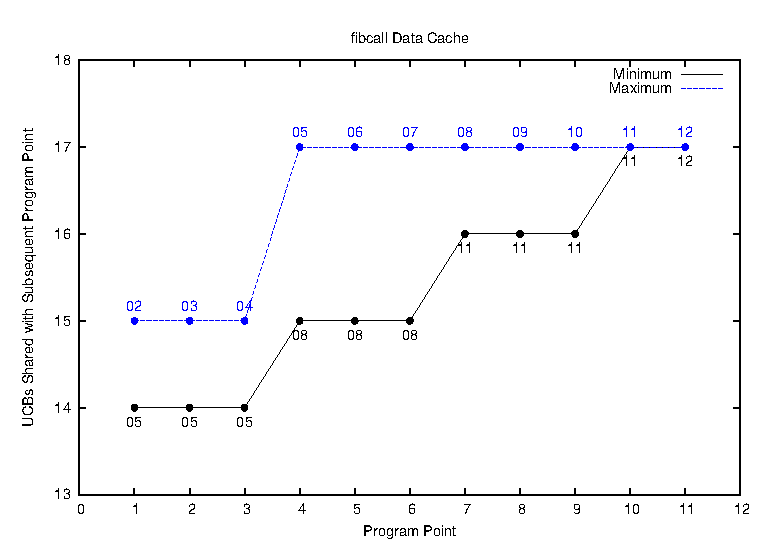
\includegraphics[width=\linewidth]{eps/fibcall-dcache.eps}
\caption{Fibcall Data Cache.}
\label{fig:fibcall_data_cache}
\end{center}
\end{figure}
%
\vspace{-20pt}
\begin{figure}[h!]
\begin{center}
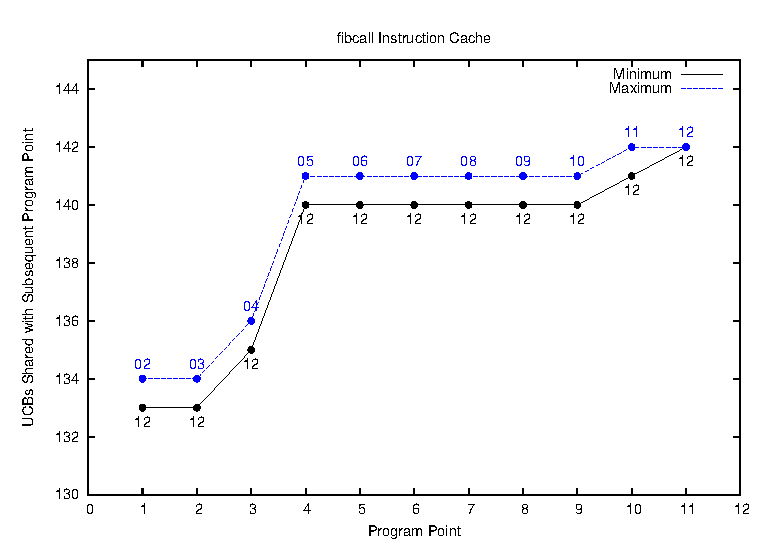
\includegraphics[width=\linewidth]{eps/fibcall-icache.eps}
\caption{Fibcall Instruction Cache.}
\label{fig:fibcall_instruction_cache}
\end{center}
\end{figure}
%
\begin{figure}[h!]
\vspace{-20pt}
\begin{center}
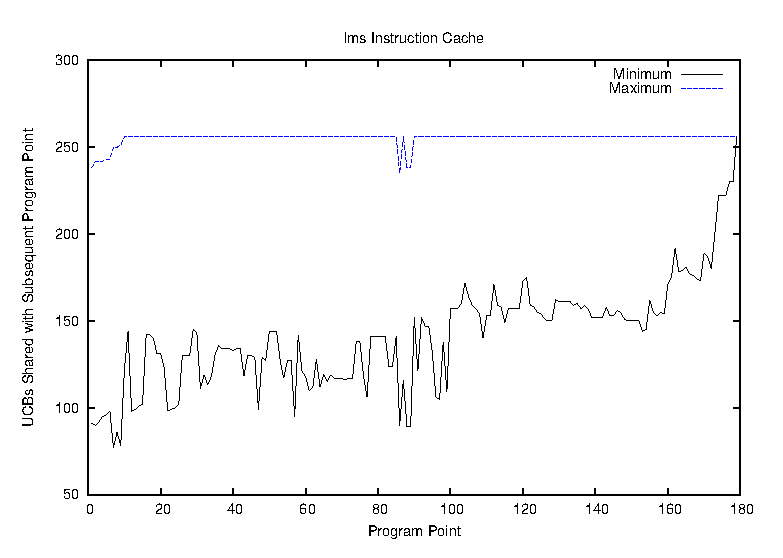
\includegraphics[width=\linewidth]{eps/lms-icache.eps}
\caption{LMS Instruction Cache.}
\label{fig:lms_instruction_cache}
\end{center}
\vspace{-10pt}
\end{figure}
%
\vspace{-20pt}
\begin{figure}[h!]
\begin{center}
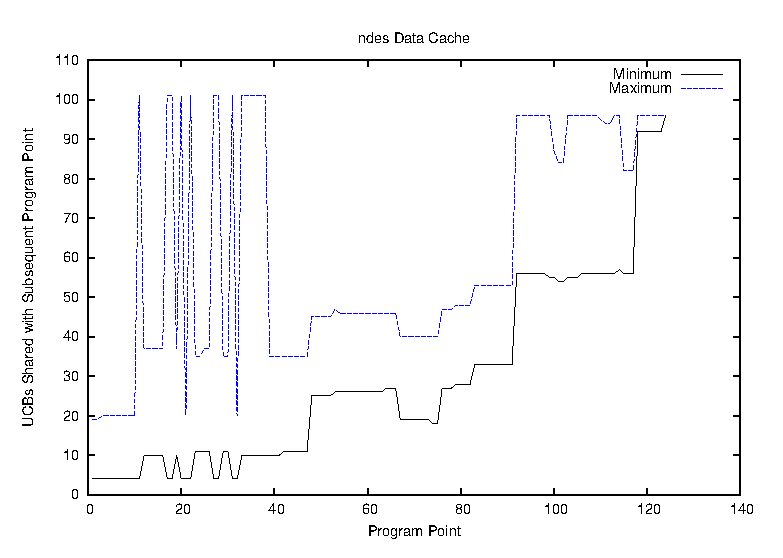
\includegraphics[width=\linewidth]{eps/ndes-dcache.eps}
\caption{NDES Data Cache.}
\label{fig:ndes_data_cache}
\end{center}
\end{figure}
%
\vspace{-20pt}
\begin{figure}[h!]
\begin{center}
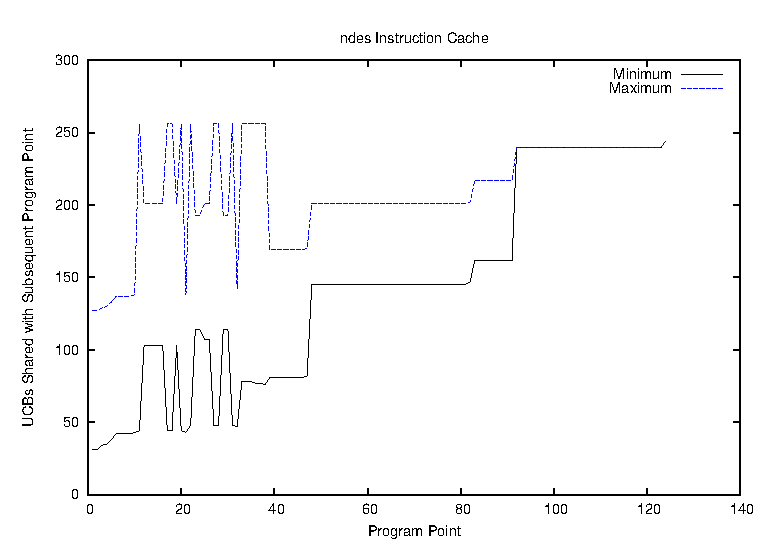
\includegraphics[width=\linewidth]{eps/ndes-icache.eps}
\caption{NDES Instruction Cache.}
\label{fig:ndes_instruction_cache}
\end{center}
\end{figure}
% 



%\scriptsize\addtolength{\baselineskip}{-2mm}
%\bibliographystyle{IEEEtran}
%\bibliography{web-bib}


%end document
\end{document}

